\documentclass{amsart}
\usepackage{amsmath,amsthm,amssymb}
\usepackage{xcolor}
\usepackage{tikz}

\begin{document}

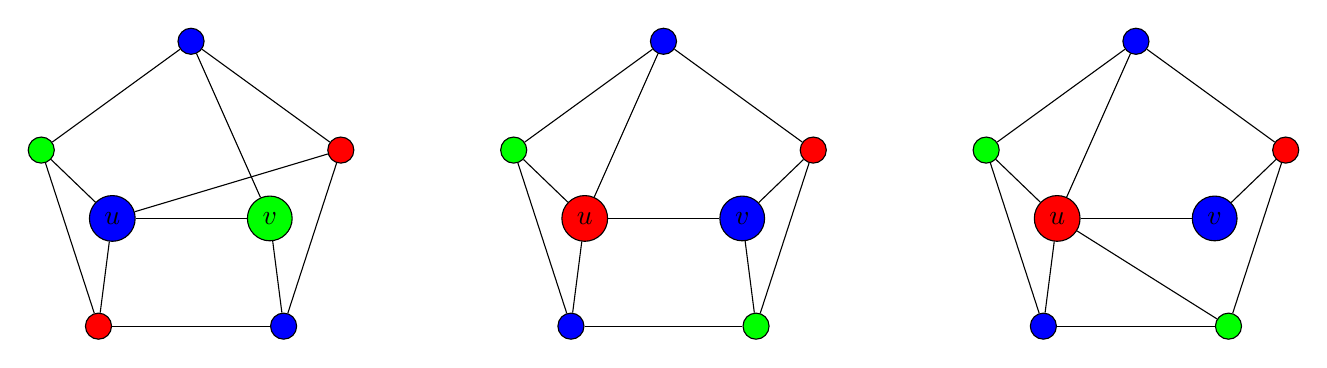
\begin{tikzpicture}
\tikzstyle{vertex}=[draw,shape=circle];

\begin{scope}

    \node[vertex,fill=blue] (a) at (90:2) {};
    \node[vertex,fill=red] (e) at (-72+90:2) {}
        edge (a);
    \node[vertex,fill=blue] (d) at (-2*72+90:2) {}
        edge (e);
    \node[vertex,fill=red] (c) at (-3*72+90:2) {}
        edge (d);
    \node[vertex,fill=green] (b) at (-4*72+90:2) {}
        edge (a)
        edge (c);
    \node[vertex,fill=blue] (u) at (-1,-0.25) {$u$}
        edge (e)
        edge (c)
        edge (b);
    \node[vertex,fill=green] (v) at (1,-0.25) {$v$}
        edge (a)
        edge (d)
        edge (u);

\end{scope}

\begin{scope}[xshift=6cm]

    \node[vertex,fill=blue] (a) at (90:2) {};
    \node[vertex,fill=red] (e) at (-72+90:2) {}
        edge (a);
    \node[vertex,fill=green] (d) at (-2*72+90:2) {}
        edge (e);
    \node[vertex,fill=blue] (c) at (-3*72+90:2) {}
        edge (d);
    \node[vertex,fill=green] (b) at (-4*72+90:2) {}
        edge (a)
        edge (c);
    \node[vertex,fill=red] (u) at (-1,-0.25) {$u$}
        edge (b)
        edge (c)
        edge (a);
    \node[vertex,fill=blue] (v) at (1,-0.25) {$v$}
        edge (d)
        edge (e)
        edge (u);

\end{scope}

\begin{scope}[xshift=12cm]

    \node[vertex,fill=blue] (a) at (90:2) {};
    \node[vertex,fill=red] (e) at (-72+90:2) {}
        edge (a);
    \node[vertex,fill=green] (d) at (-2*72+90:2) {}
        edge (e);
    \node[vertex,fill=blue] (c) at (-3*72+90:2) {}
        edge (d);
    \node[vertex,fill=green] (b) at (-4*72+90:2) {}
        edge (a)
        edge (c);
    \node[vertex,fill=red] (u) at (-1,-0.25) {$u$}
        edge (b)
        edge (c)
        edge (a)
        edge (d);
    \node[vertex,fill=blue] (v) at (1,-0.25) {$v$}
        edge (e)
        edge (u);

\end{scope}

\end{tikzpicture}

\end{document}